\chapter{Medidas e incertezas}
\label{sec:medidasErro}
\vspace{-0.5cm}

Uma das maneiras para conhecer e descrever a natureza que nos rodeia é mediante a realização de observações experimentais, que chamamos de medidas. O primeiro problema com o qual nos encontramos é como os resultados encontrados podem ser comunicados de maneira clara, de forma que sejam compreensíveis e reprodutíveis por outros experimentadores. Para estabelecer o valor de uma grandeza (mensurando) temos que utilizar instrumentos e um método de medida, como também é necessário definir as unidades da medida. Por exemplo se desejamos medir a largura de uma mesa, o instrumento de medição será uma régua ou uma trena e, utilizando o sistema de unidades internacional (SI), a unidade que utilizaremos será o metro (m). A régua, portanto, estará calibrada nessa unidade ou em seus submúltiplos, como, por exemplo, centímetros e milímetros. O método de medição consistirá em determinar quantas vezes a unidade e as frações dela estão contidas no valor do mensurando.

Toda medição é afetada por uma incerteza que provém das limitações impostas pela precisão e exatidão dos instrumentos utilizados, da interação do método de medição com o mensurando, da definição do objeto a medir, e da influência do(s) observador(es) que realiza(m) a medição.

O que se procura em cada medição é conhecer o valor medido ($x$) e a sua incerteza ($\delta_x$) na de\-ter\-mi\-na\-ção do resultado, ou seja, determinar os limites probabilísticos destas incertezas.  Procura-se estabelecer um intervalo
\begin{equation}
x - \delta_x < x < x + \delta_x
\end{equation}
\noindent
como ilustrado na Figura~\ref{fig:Inter}, dentro do qual podemos dizer que o valor da grandeza se encontra, com uma certa probabilidade.  Em geral utiliza-se como incerteza um intervalo em torno do valor central com 68\% de probabilidade. 
\begin{figure}[h]
\begin{center}
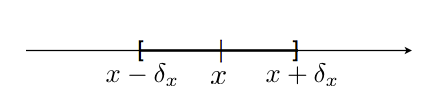
\includegraphics[width=10cm]{fig/IntervaloIncerteza}
\vspace{-0.5cm}
\caption{\label{fig:Inter} Intervalo de probabilidade para a grandeza medida, onde $x$ é o valor mais representativo da nossa medição e $\delta_x$ é a incerteza absoluta.}
\vspace{-0.5cm}
\end{center}
\end{figure}

Não existem regras para determinar o tamanho do intervalo, porque dependerá de muitos fatores do processo de medição. O tipo de medição, a figura da escala, a acuidade visual de quem esteja fazendo a medida, as condições de iluminação, etc, formarão parte na determinação da largura do intervalo de medição. A incerteza associada a uma medida deve ser determinada a cada vez que se faça a medição. Por exemplo, é comum pensar que quando fazemos uma medida com uma régua com escala graduada, a "incerteza de leitura (incerteza instrumental)" é automaticamente a metade da menor divisão. Um instrumento com divisões muito finas usado para medir um objeto com bordas mal definidas pode dar um intervalo de medição maior que várias das divisões menores. Contrariamente, um objeto bem definido com boas condições visuais pode permitir a identificação de um intervalo de medição muito menor que a menor divisão da escala. Cada situação deve ser avaliada de forma individual.
 
\vspace{-0.2 cm}
Uma forma usual de expressar o resultado de uma medição é:         
\begin{equation}
x \pm \delta_{x} 
\end{equation}
\noindent
e indicando a {\it unidade de medição}. Além disso é possível definir a {\it incerteza relativa} como:
\begin{equation}
\epsilon_x = \frac{\delta_x}{x} 
\end{equation}
\noindent
que expressa o quão significativa é a incerteza em relação a valor medido. Também pode-se calcular a {\it incerteza relativa percentual} como:
\begin{equation}
\epsilon_{\%} = \epsilon_x \cdot 100\% = \frac{\delta_x}{x} \cdot 100\% 
\end{equation}
\noindent

Por exemplo, ao medir o comprimento L de uma mesa podemos apresentá-lo como L=(1,00 $\pm$ 0,01) m ou L=1,00 $\pm$ 0,01 m, se encontramos um valor de 1,00 m, com uma incerteza de 1 cm em torno desse valor central encontrado. É importante apresentar sempre o valor central e a incerteza na mesma unidade. Essa medição tem um incerteza relativa de 0,01 (0,01/1,00) e uma incerteza relativa percentual de 1\%. A palavra {\bf precisão} muitas vezes é utilizada como sinônimo de incerteza relativa percentual. Note, no entanto, que nem sempre a precisão de uma medida corresponde à precisão do instrumento utilizado para realizá-la. A precisão de um instrumento será discutida em contraposição ao conceito de acurácia mais abaixo.
\newpage
\section*{Incertezas}
Os distintos tipos de incertezas podem ser classificados em:
\begin{itemize}
\item {\bf Incertezas do instrumento:} Os instrumentos de medição têm uma incerteza finita que está associada à variação mínima da magnitude que ele mesmo pode detectar. Por exemplo, se temos uma régua graduada em milímetros, não será possível detectar variações muito menores que uma fração de milímetro. Se, ao lermos o valor medido na régua, aproximamos para o valor inteiro em mm que mais se aproxima da medida, dizemos que a incerteza da régua é de 1 mm. Se, ao contrário, conseguimos identificar valores múltiplos de meio milímetro, então dizemos que a incerteza é de 0,5 mm. Não é, no entanto, razoável supor que conseguimos identificar a olho nú frações menores que 0,5 mm em uma régua milimetrada.

\item {\bf Incertezas estatísticas ou aleatórias:} São as devidas flutuações aleatórias na deter\-mi\-na\-ção do valor do mensurando entre uma medida e outra.  Estas flutuações ocorrem com igual probabilidade tanto para mais quanto para menos. Portanto, medindo várias vezes e calculando a média, é possível reduzir a incerteza significativamente. Estas incertezas são tratadas pela teoria estatística de erros de medição.

\item {\bf Incertezas sistemáticas:} Acontecem pelas imperfeições dos instrumentos e métodos de medição e sempre se produzem no mesmo sentido (não podem ser eliminados com várias medições). Alguns exemplos podem ser um relógio que atrasa ou adianta, uma régua que se dilata, o erro devido à paralaxe, etc... 
\end{itemize}

A interação do método de medição com o mensurando também pode introduzir erros.  Consideremos como exemplo a medição de temperatura para a qual utilizamos um ter\-mô\-me\-tro. Parte do calor do objeto que queremos medir flui ao termômetro (ou vice-versa), de maneira que o resultado da medição do valor da temperatura difere do original devido à presença do termômetro (interação que devemos realizar). Fica claro que esta interação pode ser desprezível, se, por exemplo, estamos medindo a temperatura de um litro de água, mas a quantidade de calor transferida ao termômetro pode ser significativa se a quantidade de volume é uma fração pequena de, por exemplo, um mililitro e utilizamos um termômetro convencional.

\section*{Precisão e exatidão}

A precisão de um instrumento ou um método de medida está relacionada à sensibilidade ou menor variação de uma grandeza que pode ser detectada com certo instrumento ou método. Dizemos que um paquímetro (por exemplo, com mínima divisão de 0,01 mm) é mais preciso que uma régua (mínima divisão 1 mm) ou que um cronômetro (por exemplo com mínima divisão 10 ms) é mais preciso que um relógio (mínima divisão 1 s), etc. Quanto menor a {\bf incerteza relativa} de uma medição, mais precisa ela é. É importante notar que o valor absoluto da incerteza isoladamente não  é suficiente para qualificar a precisão de uma medida. Por exemplo, reportar a distância entre Rio e São Paulo com incerteza de um metro certamente é muito bom. Por outro lado, medir o comprimento de um carro com incerteza de um metro é muito ruim. Qual a diferença? No primeiro caso, estamos falando de uma dúvida de um metro em cerca de 500 km e no segundo caso, a incerteza é de um metro em cerca de 4 metros.

Além da precisão, é importante realizar uma medição com exatidão ou, utilizando um termo mais antigo, acurácia. Esta está geralmente relacionada com a qualidade da calibração do instrumento utilizado ou o método de medição aplicado. Imaginemos que utilizamos um cronômetro para medir os tempos com uma precisão de 10 ms, mas sabemos que atrasa 1 minuto cada uma hora. Por outro lado, utilizamos um relógio com uma precisão de 1 s que marca a hora certa a todo instante. Neste caso vamos dizer que o cronômetro é o mais preciso, mas o relógio é o mais acurado. Um critério para se comparar a exatidão de duas medidas é dado pela menor discrepância relativa. A discrepância é definida como o módulo da diferença entre o valor medido e um valor de referência para a grandeza e a discrepância relativa é definida como o módulo da razão entre a discrepância e o valor de referência. Quanto menor a discrepância relativa de uma medida, mais exata ou acurada ela é.

Portanto, procuraremos sempre realizar uma medição utilizando um método que seja preciso e exato ao mesmo tempo.

